\documentclass[12pt,a4paper,twoside,times,sky,standard]{csiroreport2017}


\usepackage{amsmath,amssymb,wasysym,bm}
\newcommand{\etal}{\textit{et al.}}
\newcommand{\ds}{\displaystyle}
\newcommand{\eps}{\epsilon}
\newcommand{\rp}{r^\prime}
\newcommand{\ap}{a^\prime}
\newcommand{\lp}{l^\prime}
\newcommand{\vphi}{\varphi}
\newcommand{\ty}{\tilde{y}}
\newcommand{\tl}{\tilde{l}}
\newcommand{\tr}{\tilde{r}}
\newcommand{\tmax}{t_{\rm max}}
\newcommand{\tbz}{\tilde{\textbf{z}}}
\newcommand{\vtheta}{\vartheta}
\newcommand{\vphit}{\vphi^{\rm tag}}
\newcommand{\xtheta}{\mbox{\boldmath$\theta$}}


%Fill in the title, authors, in confidence text, etc as required.
%If you don't want one or the other then just comment them out.
%\docinconfidence[Commercial In Confidence]


\docdivision[Environment]


\docbusinessunit[
    CSIRO Environment\\
    Battery Point, Hobart 7000, Tasmania, Australia.\\
]


% The title of the document. Try to keep it to 3 lines or less.

\doctitle[\vspace{0mm}\huge Initial exploration of replacing the CCAMLR rule for Macquarie Island toothfish]

\docfootertitle[MITF initial MSE]

\docauthors[\vspace{4mm}\Large R. Hillary \& P. Bessell-Browne]

%\docreportnum[Report Number: CMIS 2009/00]

\docreportdate[26\textsuperscript{th} April 2024]

\doccopyrightyear[2024] % For the Copyright and Disclaimer notice


\begin{document}
%=================================================

\section{Background}

The Macquarie Island Patagonian toothfish fishery, as well as the majority of the CCAMLR-managed toothfish fisheries (HIMI, South Georgia, Ross Sea), are all managed via integrated stock assessments that are then used to generate an overall TAC via the CCAMLR Harvest Control Rule (HCR) - henceforth ``the CCAMLR rule''. The general working mechanism of the CCAMLR rule can be summarised as follows:

\begin{enumerate}
    \item Use current state of population from assessment to project forward
    \item Calculate (constant) catch where relative SSB above 50 with probability 0.5 after 35 years
    \item Calculate (constant) catch where relative SSB above 20\% with probability 0.9 (all years)
    \item TAC is the \emph{lowest} of these two catches
\end{enumerate}

The initial context of the rule could be characterised as follows: given sporadic estimates of the abundance of a population, how can precautionary catch levels be set in place - possibly for an extended amount of time. Within the Australian fisheries context the CCAMLR rule as been applied consistently for over a decade for both the HIMI and Macquarie Island fisheries. The original context for the CCAMLR rule does not really apply to the current state of Australian toothfish fisheries. Both the major fisheries have mature, relatively complex integrated assessments that are capable of providing multi-decade reconstructions of both the population and fishery dynamics. They both have their advantages and challenges - and some of these layer onto the overall effectiveness of the CCAMLR management approach - but they have little in common with the original CCAMLR rule context. More importantly, the application of the rule has resulted in a number of negative performance behaviours:

\begin{itemize}
    \item TAC variability - there are no explicit constraints on the degree to which the TAC can vary from one decision to the next. Changes in excess of 20\% are quite common. This level of change is often hard-wired into other management procedures as a \emph{maximum} change and values well below this are considered good performance indicators
    \item Interaction with recent population dynamics - the constant catch, long-term projection nature of the CCAMLR rule has the tendency to amplify the effect of recent stock and fishery dynamics on the TAC
    \item Overall it is \emph{very} sensitive to the overall scale of the population coming from the stock assessment - at least in the last three TAC decisions at Macquarie Island this relationship has been almost a one-to-one positive relationship
\end{itemize}

The last point has further implications that are hard to quantify in relation to the TAC, but very impactful in relation to the management process. If the management advice is so strongly dependent on the stock assessment it becomes scientifically and practically very difficult to explore development and adaption of the assessment where the implications for the management advice are not influencing the process - both consciously and subconsciously. As important is the fact that the CCAMLR rule has never really been fully tested in the Management Strategy Evaluation (MSE) sense, where the full feedback dynamics of the whole system are simulated. 

The process of MSE is considered best practice when developing and evaluating fisheries management strategies \cite{mse}. Since its genesis in the International Whaling Commission \cite{iwc} it has shown repeatedly that two general observations hold true: (i) ``on paper'' good ideas for management strategies do not always work very well when tested against reality; and (ii) complex is not always better than simple in terms of ``assessment'' methods in management strategies - empirical or simpler model-based assessments often out-perform the current stock assessment model when tested concurrently. A schematic of the MSE process in a systems analysis sense can be seen in Figure 1.1

\begin{figure}[hb]
    \begin{center}
        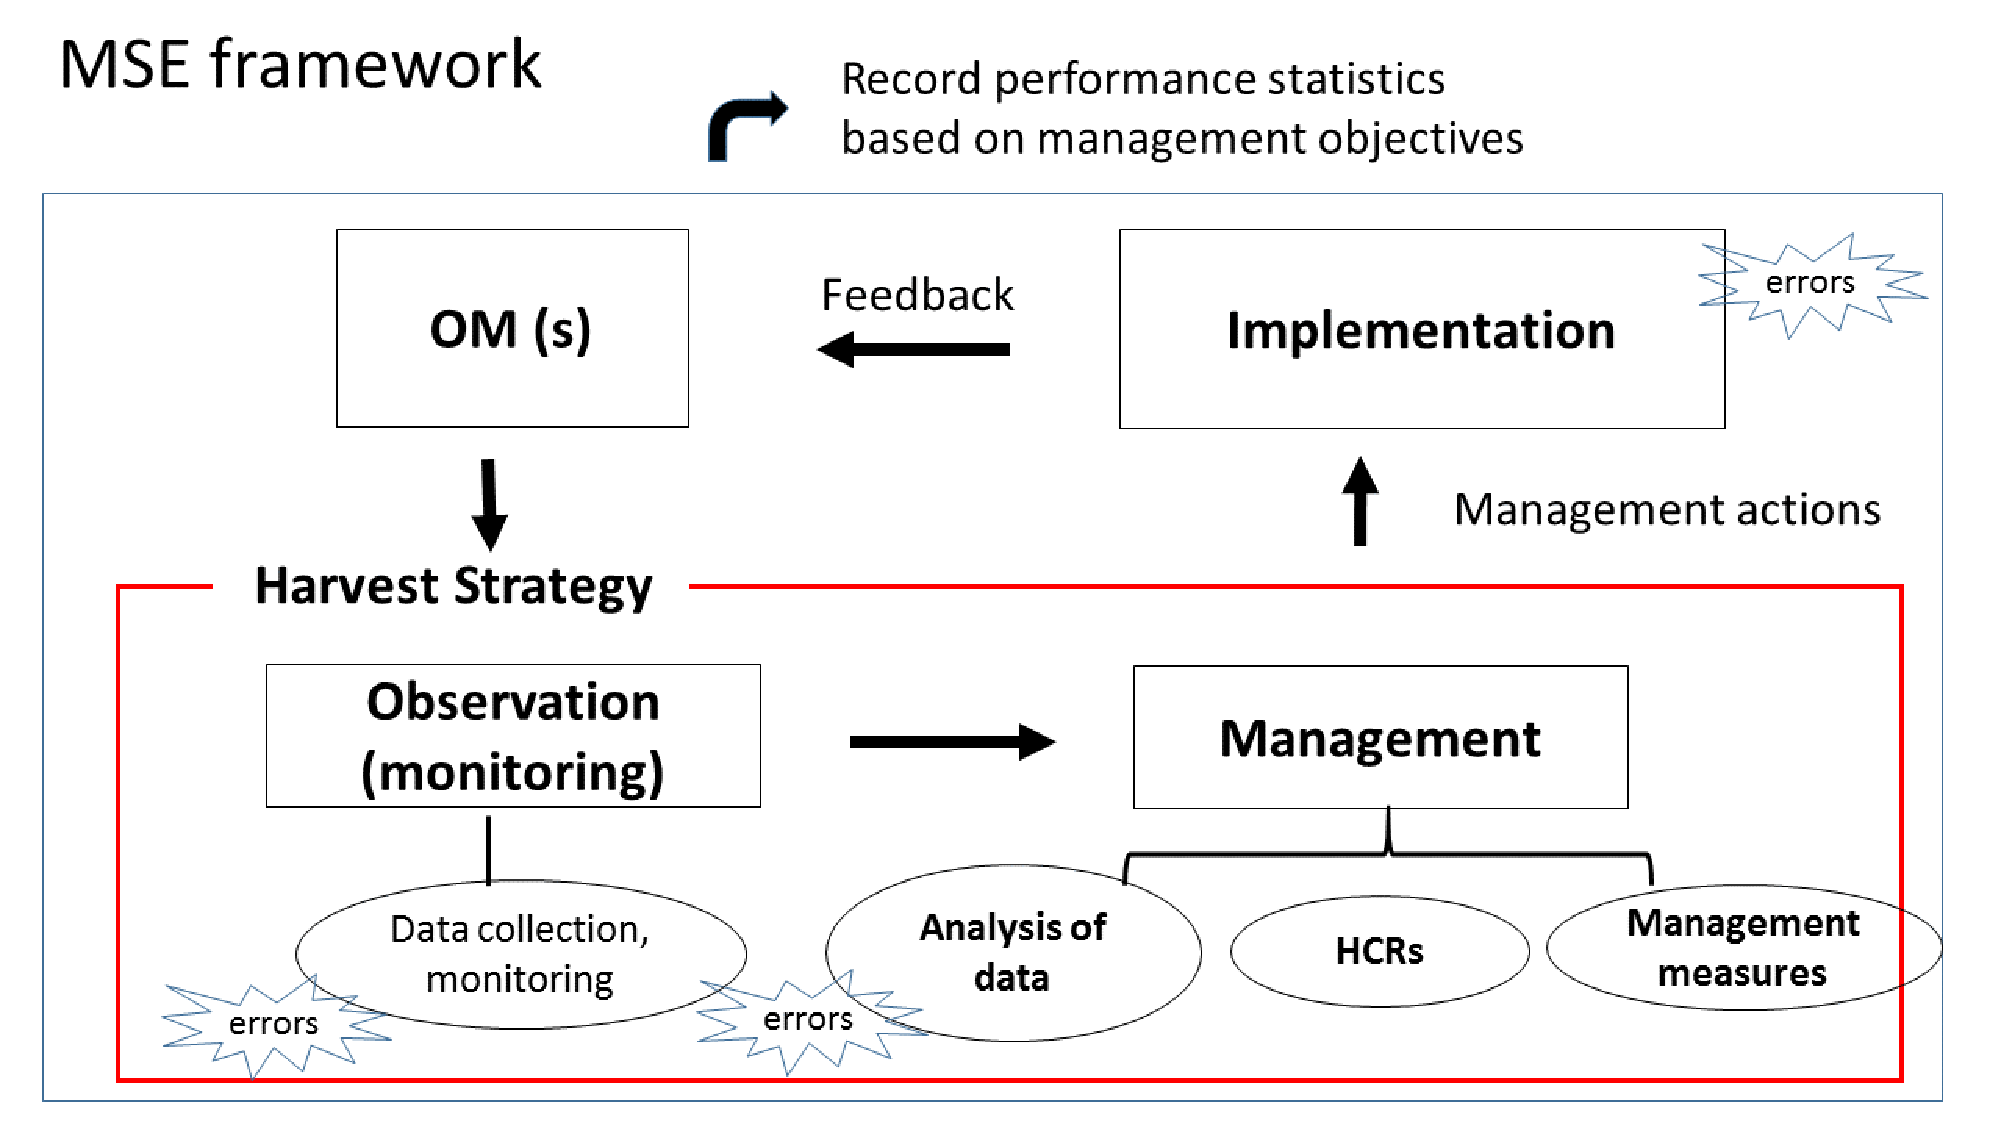
\includegraphics[width=11cm,height=7cm]{figs/MSE.pdf}
    \end{center}
    \caption{\textit{A system scale schematic of the MSE process. The red box encapsulates where the Management Procedure (harvest strategy) is embedded in the wider fishery system.}}
\end{figure}

This document is an initial exploration of what type of candidate Management Procedures (MPs) might be developed to replace the current CCAMLR approach (integrated stock assessment then use the CCAMLR rule). For Macquarie Island the major information source in relation to abundance and mortality is the tagging data, with additional key information from the age, length and maturity data. The stock assessment statistically integrates all these data sources to provide us with an estimated spatiotemporal reconstruction of the population and fishery dynamics for the resource \cite{misa}. Research from a large diversity of MSE examples and contexts \cite{mse,iwc,sbtmp,mprev} all give credence to the idea that either empirical or model-based MPs that are notably less complex than the stock assessment can not only perform well in managing a fishery, but can often perform \emph{better} than the stock assessment in this regard. In this initial tranche of MSE work we posit that the tagging data are the best candidate for a \emph{single} data set that could be used in a suite of candidate MPs. This does not suggest that there may not be additional beneficial information from the additional data (age and length composition) - this is clearly demonstrated in the stock assessment model \cite{misa}. However, the assessment also tells us that the dominant data set in relation to estimates of abundance and mortality is the mark-recapture data. So, while we do not rule out exploring the utility of including additional data as inputs to candidate MPs, the MPs proposed herein use \emph{only} the tagging data.

\section{Methods}

There are a number of general steps in a fully realised MSE loop:

\begin{itemize}
    \item Definition and conditioning of suite of Operating Models (OMs) that will generate population and fishery dynamics as well as the observations to be used in the candidate MPs
    \item Definition of the candidate MPs: (i) suite of input data; (ii) underlying ``assessment'' model; and (iii) HCR that uses assessment output and additional parameters to generate the relevant management action variable (e.g. TAC)
    \item A set of key management objectives for the candidate MPs to achieve and a suite of performance criteria against which we can assess relative performance across the candidate MPs
    \item A suite of past and/or future additional scenarios (a.k.a. robustness tests) to ascertain how robust the candidate MPs, which can acceptably achieve the key management objectives, are to alternate hypotheses about the state of the system under consideration  
\end{itemize}

\subsection{Operating Model structures}

Generally, OMs require \emph{at least} the nominal level of complexity of the stock assessment if one exists \cite{mse} but ideally they should have the capability of being able to model dynamics that are often far more complicated than the assessment. Features such as time/sex/size/age varying processes (e.g. growth, natural mortality, selectivity, migration) not modelled in the assessment are often included so as to be able to simulate the kind of features we want a candidate MP to be robust to. The OM needs to (i) simulate the population and fishery dynamics in response to population (endogenous) and environmental (exogenous) factors, and the exploitation of the resource by the fishery; and (ii) simulate the suite of observations we intend to use in the candidate MPs.

The population dynamics in the OMs we employ are year/age/length/sex/spatial in general structure, as is the stock assessment \cite{misa}, with the additional capability to permit temporal structure in various population (recruitment, natural mortality, growth) and fishery (selectivity, fishing location) processes. It can also accommodate sex/age/size structure in processes such as natural mortality and migration if required. For the data simulation part of the OM we need to define a suitable suite of observation error models. These connect the population and fishery dynamics to an appropriate generating probability distribution. Within the MSE software suite we can generate:

\begin{itemize}
    \item Mark-recapture data: focus is on tag release covariate conditional estimators (the Brownie suite of models) so this is how they are simulated (with over-dispersion included) in the observation error model
    \item Length data: length composition by fishery via the Dirichlet-multinomial
    \item Age-given-length data: by fishery via the multinomial distribution
    \item Relative abundance indices: surveys, fleet-specific CPUE indices via either the multivariate or simpler log-normal distribution
\end{itemize}

For the simulation of the tag data the probabilities we model the tag release dynamics of each release ``event'' i.e. all the releases in a given year, sex, age class and spatial region. The probability of recapturing a tag depends on tag shedding and mortality, natural mortality, the harvest rate, and the spatial transition matrix. Though the underlying generating distribution is assumed to be a Dirichlet-multinomial we use the conditional beta-binomial generating method. This is because as we move forward in time we are releasing tags in a given release ``cohort'', recapturing them, using the data in a TAC decision year but also recapturing the same release further ahead in time. So we cannot simply use the Dirichlet-multinomial distribution to simulate the data - instead we use the beta-binomial distribution to simulate recaptures in the given time period, and as we project forward in time we use the conditional sampling approach to simulate future recaptures in the same release group. This preserves both the marginal distributions of each possible recapture event, as well as the implicit negative correlation in the multinomial (more/less recaptures ``early'' means less/more recaptures probable ``later''). The tag release age distribution is statistically inferred from the actual size distribution of animals at Macquarie Island (in this case) using the length-at-age distribution (by sex), and the number of releases is dictated by an assumed tag-per-tonne release rate, the catches by region, and the estimated sex and age distribution of releases.

\subsection{Mark-recapture estimators}

There are several main groups of tag estimators (and variations within each) but for Macquarie Island toothfish the two main groupings have been the modified Petersen (Stock Synthesis) and the Brownie - the spatial sex and length structured Brownie is used the current assessment \cite{revass2019}. The reason for moving to the spatial Brownie approach to modelling the tagging data was driven by the side-by-side comparison of the Stock Synthesis approach (two-stage negative binomial and spatial multinomial) and spatial Brownie focussed on the relative accuracy of their estimates of both spawning abundance and migration rates \cite{tagdes}.

The Brownie estimator is release conditional and it models the future recapture of tagged animals only within a given release event - it doesn't model pooled tag releases and recaptures as some Petersen-style estimators. The probability of recapturing a released tag is constructed via a two-stage process:

\begin{enumerate}
    \item Calculate the probability that a tagged fish survives the tag release process, still has \emph{at least} one tag still attached, survives both natural mortality and fishing \emph{and} is located in the spatial region of interest
    \item Conditional on the first probability, calculate the probability that the tag is recaptured \emph{and} reported
\end{enumerate}

For the spatial Brownie estimators we propose to use for the candidate MPs the structure is simplified by removing the dependence on either age (length) or sex of release as is done in the stock assessment. Additionally we also explore non-spatial estimators even if there is underlying spatial structure in the population dynamics and underlying mark-recapture data. By simplifying in this way (removing the dependence on age/length/sex at release) what these estimators are estimating will be close to what the average harvest rates would be coming from the stock assessment. The mathematical and statistical details of the suite of mark-recapture estimators can be found in the Appendix. It is not essential to obtain unbiased estimates of the true harvest rates - what matters is that there is a close correlation between the true harvest rates and those coming from the mark-recapture estimators. The process of tuning key HCR parameters can deal with any average bias and so if the estimates correlate well with the true values then any candidate MP should have useful estimates of the true harvest rate(s). All the mark-recapture estimators were coded in Template Model Builder \texttt{TMB} \cite{tmb} - the \texttt{R} package used to code the integrated stock assessment.

\subsection{Candidate Management Procedures}

There are two main derived quantities coming from the mark-recapture estimators and other fishery data:

\begin{enumerate}
    \item Harvest rates: overall/spatially averaged, $h_y$, or spatially explicit, $h_{y,r}$
    \item Exploitable abundance/biomass: given catch numbers/biomass, $C_y$, the exploitable abundance/biomass can simply be calculated by $X_y=C_y/h_y$ or $X_{y,r}=C_{y,r}/h_{y,r}$ in the spatial case and $X_y=\sum_r X_{y,r}$
\end{enumerate}

In very general terms these two variables present where the stock is ``going'' (harvest rates) and where the stock is ``at'' (exploitable abundance). In practice we could use both of these variables or just one in a candidate MP - for example the ``classic'' $\{F,SSB\}$ hockey-stick HCR used in for example the SESSF, EU and elsewhere can be mirrored to a degree using an analogous $\{h,X\}$ HCR. In practice, there are several reasons why these types of rules don't always perform as well as other often simpler approaches, but one can explore what might be termed familiar types of HCR using the estimates from the mark-recapture models.

In this initial work we explored a relatively straightforward general framework for the HCR in a given management decision year, $y$:

\begin{equation*}
    \ds TAC_{y+1}=TAC_y\times\Delta_y
\end{equation*}
where the TAC change is defined by
\begin{equation*}
    \ds \Delta_y=\min\{1+\delta_{\rm max},f(h,X,\xtheta)\}
\end{equation*}
if $\Delta_y>1$ and 
\begin{equation*}
    \ds \Delta_y=\max\{1-\delta_{\rm max},f(h,X,\xtheta)\}
\end{equation*}
if $\Delta_y<1$ and $f(h,X,\xtheta)$ is the HCR response function (with HCR parameters $\xtheta$) but the TAC change in a given decision year is bounded by $1\pm\delta_{\rm max}$. The built-in feature of this type of overall HCR an innate level of TAC stability and consistency given the next TAC is always constrained to be some maximum distance from the current one. 

One of the simplest HCRs we can construct is a target-based HCR based on the recent mean harvest rate. Define a recent moving average harvest rate as follows:
\begin{equation*}
    \ds \bar{h}=\sum\limits_{i=y-\tau+1}^y h_y,
\end{equation*}
where $\tau$ is the length of time over which the moving average is taken. Also define a ``target'' harvest rate $h^{\rm targ}$, then our HCR response function can be defined as
\begin{equation*}
    \ds f(h,\xtheta)=\left(\frac{h^{\rm targ}}{\bar{h}}\right)^\nu
\end{equation*}
so $\xtheta=\{h^{\rm targ},\nu,\tau\}$ and $\nu$ is a response parameter such that for $\nu>1$ the HCR is superlinear and for $\nu<1$ it is sublinear in its response. Initially we simply explore $\nu=1$ but there are often cases where we want to dial up (or down) the responsiveness of the HCR and this kind of parameter is a straightforward and interpretable way to do this. This type of HCR will increase/decrease the TAC if the recent mean harvest rates are below/above the target. The main tuning parameter in this HCR would be the target harvest rate, $h^{\rm targ}$ - to be clear this is just a parameter of the HCR, not a feature of the true dynamics of the OM. Even if we set the main objective to be attaining $SSB_{\rm msy}$ and tuned this MP to achieve that objective it does not mean that $h^{\rm targ}\equiv h_{\rm msy}$. Parameters of any HCR are useful degrees of freedom that can be altered or tuned directly to achieve a given set of objectives or performance characteristics and do not need to have interpretable counterparts in concepts like MSY or MEY for example, even if they are tuned to achieve those objectives. 

\subsection{Management objectives \& performance statistics}

Even in data poor settings, it is important to clearly specify a single objective (or set of multiple objectives) for candidate MPs to achieve as a base level of performance \cite{mse}. Once those objectives are set we then need a suite of performance statistics against which we can ascertain relative performance across candidate MPs. Ideally both these processes - setting objectives and deciding performance measures - should be guided by practitioners but driven strongly by policy makers and stakeholders. To obtain stakeholder buy-in and commitment to an MP it should be these groups that decide what they want an MP to achieve, and what kinds of behaviours they would like to see in the candidate MPs in \emph{how} they achieve the objectives. 

For this initial work we explored a simple management objective that the candidate MPs had to be tuned to: attain a (female) spawning stock biomass of 50\% of the unfished level with probability 0.5 at some pre-defined year (or set of years) in the future after the implementation of the MP. In terms of performance statistics there are obviously many that could be envisage but some very common ones are:

\begin{itemize}
  \item Probability that the (female) SSB falls below a given limit reference point (LRP) if one exists
  \item Average TACs for different future time periods
  \item Average annual variation (AAV) in TAC - often expressed as a percentage and the mean percentage change in TAC when a management decision is made
  \item The potential trade-off between average TAC and AAV - often they are negatively correlated (more flexible MPS can attain higher TACs but do so at the cost of more variability in TAC)
  \item Proportion of times a TAC decision triggers the maximum change condition - if this is high our MP is approximating a discrete switch function and is probably too responsive to the inputs
  \item Some kind of fishery efficiency performance statistics such as CPUE or inferred effort - or even profitability measures if some basic economic data are available
\end{itemize}

There are obviously many more that can be explored and the general rule is this: if we simulate it we can summarise it, but don't create too crowded a performance picture as it can be hard to make inferences with too many statistics.

\subsection{Robustness tests}

The general process of tuning an MP \cite{mse,sbtmp} is twofold:

\begin{enumerate}
    \item To ensure that - at least - all candidate MPs can achieve the state management objectives
    \item To ensure a level playing field between candidate MPs so that one can better assess their performance characteristics given they all have to achieve a specific management objective
\end{enumerate}

Once we have tuned a suite of candidate MPs, and inspected the performance statistics to assess any performance differences between them, the next stage in the MSE process is to see how robust they are to alternate hypotheses about the stock dynamics. Generally, the most likely suite of parameter and process hypotheses is included in the reference set of OMs used to tune the candidate MPs \cite{mse,sbtmp}. The robustness tests tend to include less likely scenarios - less supported by the data, for historic processes, or future scenarios that have not yet been seen but are considered plausible or important.

Somewhat naturally these tests separate into fishery and population dynamic groupings. In the Southern bluefin tuna example \cite{sbtmp} fishery robustness tests focussed on alternative hypotheses about past and future longline catchability (CPUE index is used in the MP) and the relationship between abundance and CPUE. Population dynamic scenarios related to future recruitment failure (given a previous prolonged period of low recruitment in the recent past) and alternative abundance indices that resulted in different stock status outcomes in the historical dynamics. 

For the Macquarie Island case there are not too many obvious fishery related robustness tests beyond fishing location dynamics (relative to the North/South divide). There is a single boat and we do not use effort directly or CPUE as an abundance index so no catchability issues to explore beyond perhaps in performance statistics. In terms of population dynamics there are some focal points: (i) size/age structured migration and changes over time given we have a spatial model; (ii) future changes in growth given observed shifts in weight-at-length in relation to possible environmental changes; (iii) future changes in recruitment dynamics (spatial split, regime changes in the average level). The MSE process is a more natural place to deal with the issue of climate change and sustainability because environmental effects are hard to include directly in the stock assessment process, and often really involve future scenarios relating to the population dynamics.

\subsection{Simple example}

To demonstrate the MSE process we employed a Macquarie Island toothfish like example case study:

\begin{itemize}
    \item Essentially the same life-history parameters (growth, maturity, natural mortality), fishery characteristics (long-line, selectivity parameters), and spatial set up (two areas with 10\% annual movement for all ages)
    \item The population begins at the unfished state with a fixed harvest rate fishing strategy for 20 years before the MP is implemented. The fixed harvest rate is the value that will attain a female SSB depletion level of 0.5 at deterministic equilibrium
    \item Ten years after fishing commenced an annual tagging program at 3 tags-per-tonne is initiated 
    \item After twenty years of fishing when the tagging data has sufficiently accumulated we assume an MP is implemented with a TAC decision made every 5 years
    \item The projection goes for 20 years and the candidate MPs are tuned achieve a female SSB level of 50\% of unfished with probability 0.5 in the final year of the projections (i.e. 20 years after MP implementation)
\end{itemize}

This is a simple almost exploratory fisheries scenario but it is a useful  in that it can outline several key features of relevance to the Macquarie Island fishery. In terms of candidate MPs we explored two:

\begin{enumerate}
    \item \textbf{MP1}: uses spatially/sex/age aggregated tagging data using the non-spatial mark-recapture estimator and estimates the random effect variance of the harvest rate year effects. The fixed HCR parameters are $\tau=4$ and $\nu=1$ with $h^{\rm targ}$ the tuning parameter
    \item \textbf{MP2}: uses sex/age aggregated but spatially structured tagging data using the spatial mark-recpature estimator (estimating area-specific harvest rates and migration parameters jointly)  with the random effect variance of the harvest rate year effects estimated also. To get an overall harvest rate the MP uses an average of the region-specific harvest rates (weighted by the relative catch split). The fixed HCR parameters are $\tau=4$ and $\nu=1$ with $h^{\rm targ}$ the tuning parameter
\end{enumerate}

\section{Results}

As well as summarising the initial example MSE scenario in this section we also outline how well the two main non-spatial and spatial mark-recapture estimators perform on the actual Macquarie Island toothfish fishery tagging data. This is to demonstrate that these simplified estimators can go along way to replicating the key features of the estimates of harvest rates (and migration in the spatial case) coming from the stock assessment. 

\subsection{Example MSE results}

Both \textbf{MP1} \& \textbf{MP2} were tuned (via the $h^{\rm targ}$ HCR parameter) to meet the example management objectives. We summarised their performance using five main statistics:

\begin{enumerate}
    \item Relative (female) SSB in the middle of the projection period (10 years from the implementation of the candidate MPs)
    \item Relative (female) SSB at the end of the projection period (20 years from the implementation of the candidate MPs)
    \item Time-averaged TAC for the projection period after MP implementation
    \item The AAV in the projection period when the MP is active
    \item The probability that the maximum TAC change constraint is triggered in the active MP projection period
\end{enumerate}

Figure 3.1 summarises the performance statistics we calculated for the two candidate MPs. Clearly the performance of the two candidate MPs is very similar. They are both tuned, within a tolerance of 1\%, to obtain the same final relative SSB and we see a very similar distribution around the tuned median depletion at the end of the projection period. In terms of average TACs the medians are very similar - a little higher for \textbf{MP2} but also a little more variable - as are the AAV statistics, though for \textbf{MP2} the distribution is a little narrower. The probability that the maximum TAC change constraint was triggered for \textbf{MP1} and \textbf{MP2} was and 0.015 and 0.011,respectively.

\begin{figure}[hb]
    \begin{center}
        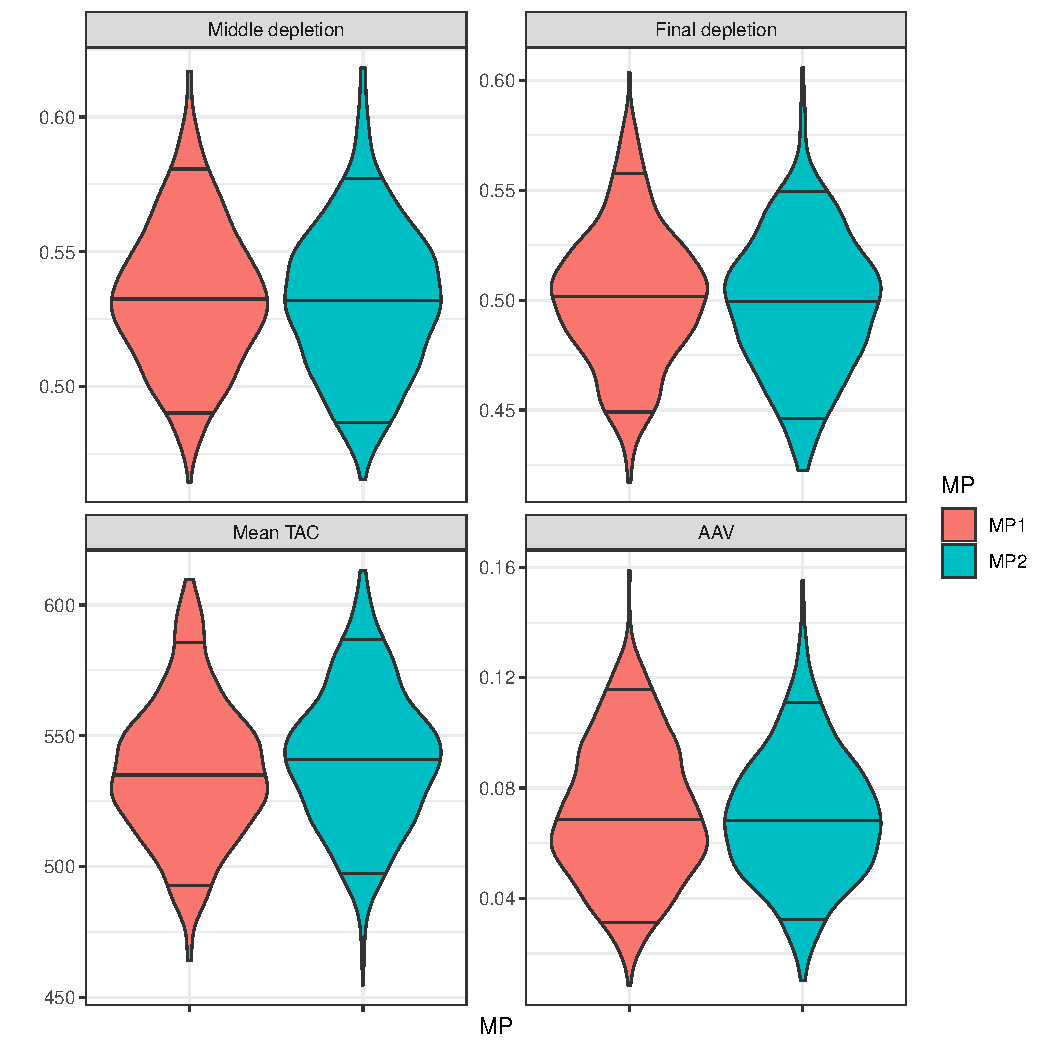
\includegraphics[width=11cm,height=10cm]{figs/fixedh_mpcomp.pdf}
    \end{center}
    \caption{\textit{Performance summary of the two tuned candidate MPs. The quantiles within the violins are the median and approximate 90\%iles.}}
\end{figure}

Figure 3.2 graphically summarises the time evolution of the key population and fishery dynamics: relative female SSB, TAC and average harvest rates. We only show them for \textbf{MP1} given they are very similar for \textbf{MP2}.

\begin{figure}[hb]
    \begin{center}
        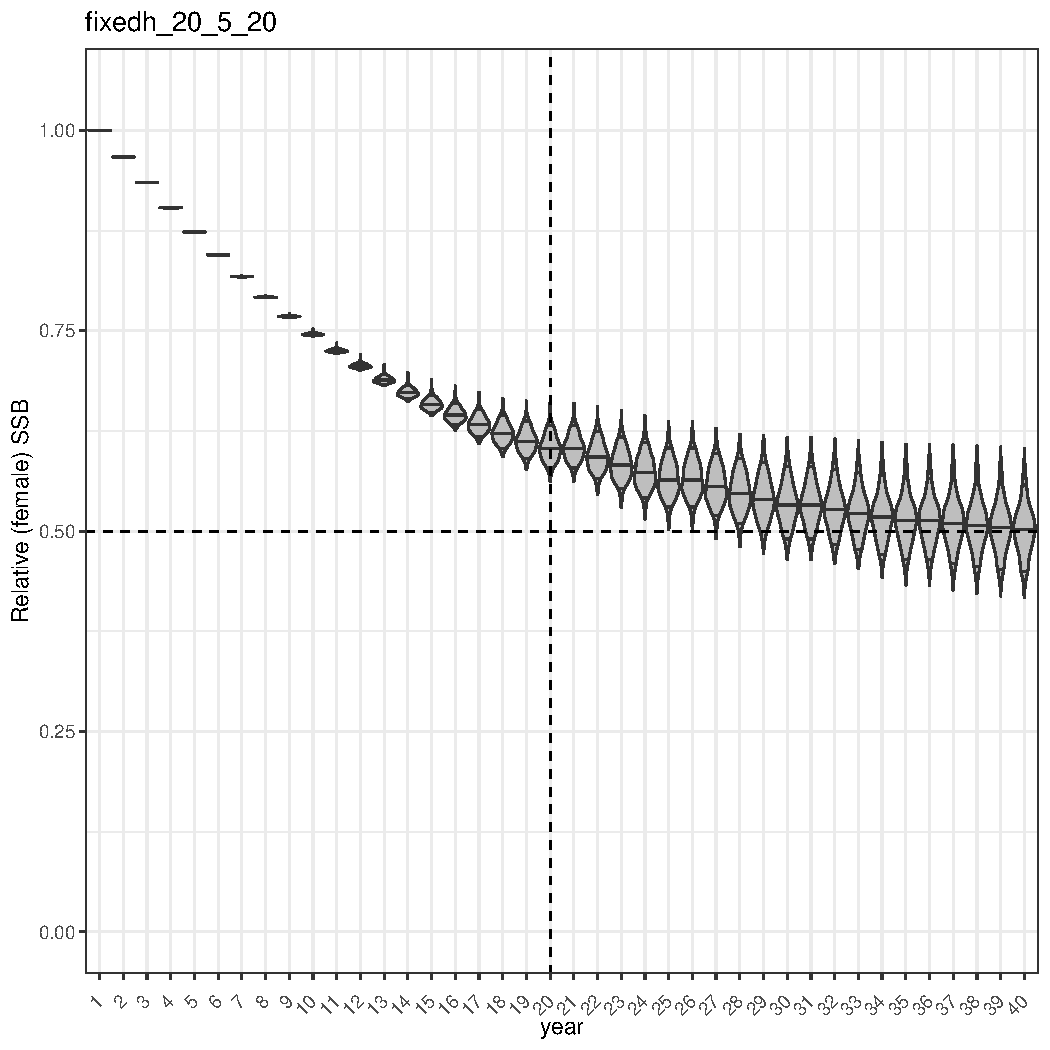
\includegraphics[width=5cm,height=5cm]{figs/fixedh_dep.pdf}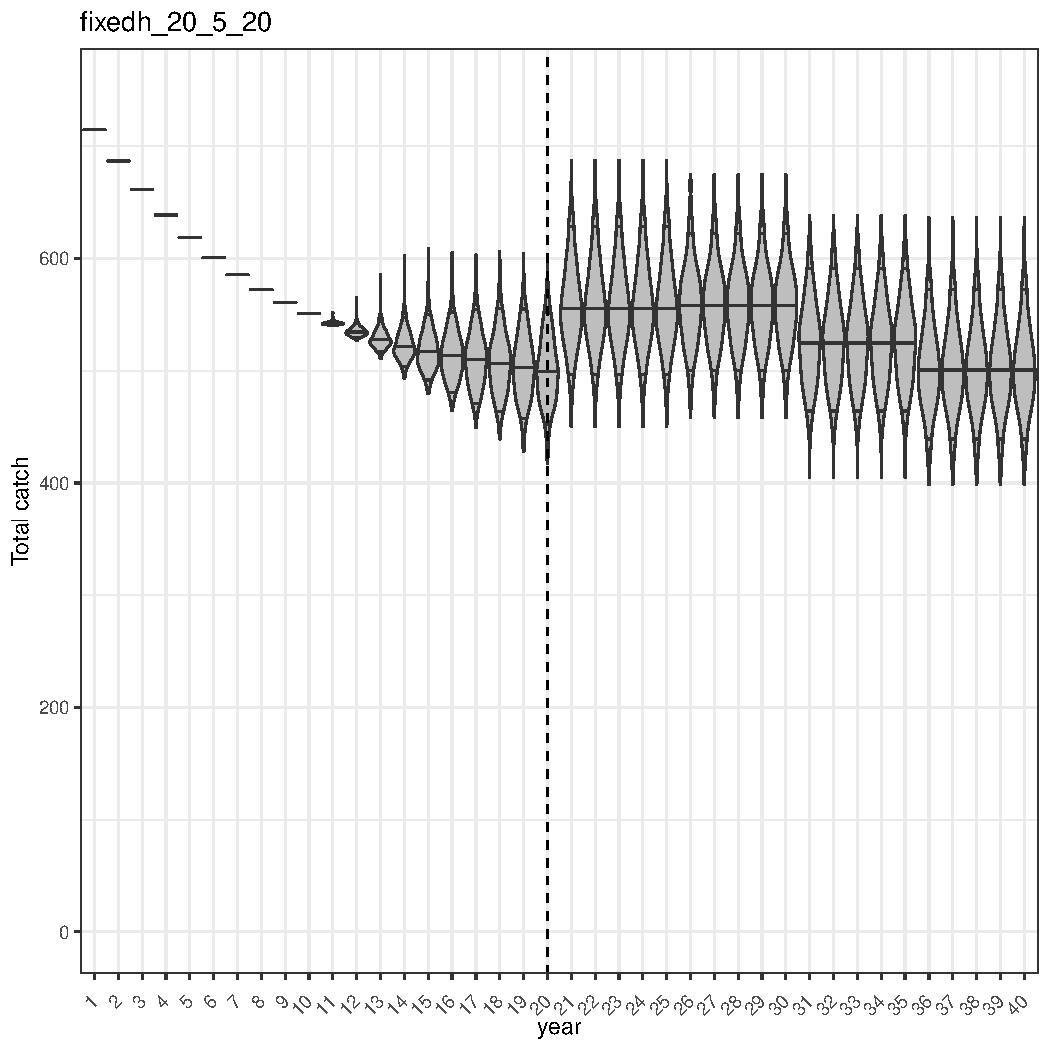
\includegraphics[width=5cm,height=5cm]{figs/fixedh_tac.pdf}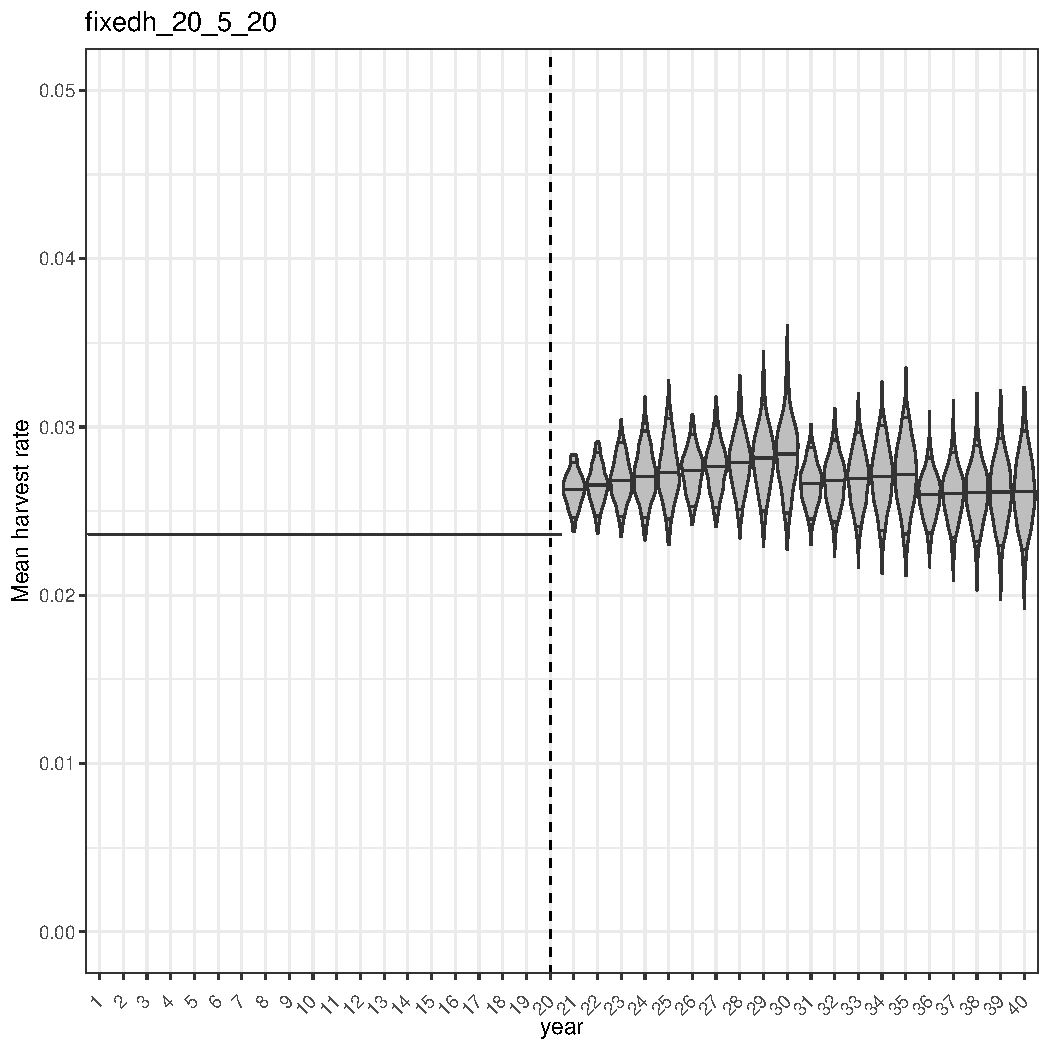
\includegraphics[width=5cm,height=5cm]{figs/fixedh_hrate.pdf}
    \end{center}
    \caption{\textit{Time evolution summary of the relative female SSB (left), TAC (middle), and the average harvest rate (right). The quantiles within the violins are the median and approximate 90\%iles.}}
\end{figure}


\subsection{Tagging estimators and Macquarie Island tagging data}

\section{Discussion}

\clearpage
\begin{thebibliography}{99}

    \bibitem{mse} Punt, A.E. \etal~(2016) Management strategy evaluation: best practices. \textit{Fish \& Fisheries} {\bf 70}: 303--334.

    \bibitem{iwc} Cooke, J.G. (1999) Improvement of fishery-management advice through simulation testing of harvest algorithms. \textit{ICES J. Mar. Sci.} {\bf 56}: 797--810.

    \bibitem{misa} Bessell-Browne, P., and Hillary, R.M. (2023) Integrated stock assessment for Macquarie Island toothfish using data upto and including
        2022. \textit{SARAG May 2023}.

    \bibitem{sbtmp} Hillary, R.M. \etal (2016) A scientific alternative to moratoria for rebuilding depleted international tuna stocks. \textit{Fish \& Fisheries} {\bf 17}: 469--482.

    \bibitem{mprev} Carruthers, T.R. (2016) Performance review of simple management procedures. \textit{ICES. J. Mar. Sci.} {\bf 73}(2): 464--482.

    \bibitem{revass2019} Proposed new assessment structure for Macquarie Island toothfish using data upto and including August 2018. \textit{SARAG 59}.

    \bibitem{tagdes} Hillary, R. M. and Day, J. (2017) Impact of spatial tagging rates for key estimates coming from the Macquarie Island toothfish assessment. \textit{SARAG 56}.

    \bibitem{tmb} Kristensen, K. \etal~(2016) TMB: Automatic Differentiation and Laplace Approximation. \textit{J. Stat. Soft.} {\bf 70}(5): 1--21.

\end{thebibliography}

\clearpage

\section*{Appendix}

\end{document}
